%  article.tex (Version 3.3, released 19 January 2008)
%  Article to demonstrate format for SPIE Proceedings
%  Special instructions are included in this file after the
%  symbol %>>>>
%  Numerous commands are commented out, but included to show how
%  to effect various options, e.g., to print page numbers, etc.
%  This LaTeX source file is composed for LaTeX2e.

%  The following commands have been added in the SPIE class 
%  file (spie.cls) and will not be understood in other classes:
%  \supit{}, \authorinfo{}, \skiplinehalf, \keywords{}
%  The bibliography style file is called spiebib.bst, 
%  which replaces the standard style unstr.bst.  

\documentclass[]{spie}  %>>> use for US letter paper
%%\documentclass[a4paper]{spie}  %>>> use this instead for A4 paper
%%\documentclass[nocompress]{spie}  %>>> to avoid compression of citations
%% \addtolength{\voffset}{9mm}   %>>> moves text field down
%% \renewcommand{\baselinestretch}{1.65}   %>>> 1.65 for double spacing, 1.25 for 1.5 spacing 
%  The following command loads a graphics package to include images 
%  in the document. It may be necessary to specify a DVI driver option,
%  e.g., [dvips], but that may be inappropriate for some LaTeX 
%  installations.
\usepackage[brazil]{babel}
\usepackage[utf8]{inputenc}
\usepackage{amsfonts}
\usepackage{amssymb}
\usepackage{amsmath}
\usepackage[]{graphicx}
\usepackage{hyperref}
\usepackage{subcaption}
\usepackage{float}
\usepackage{cite}


\title{Comparação entre os metodos de registro Demons e Thin Plate Splines aplicados a imagens médicas} 

%>>>> The author is responsible for formatting the 
%  author list and their institutions.  Use  \skiplinehalf 
%  to separate author list from addresses and between each address.
%  The correspondence between each author and his/her address
%  can be indicated with a superscript in italics, 
%  which is easily obtained with \supit{}.

\author{Thiago de Gouveia Nunes\supit{1}
\skiplinehalf
\supit{1}IME-USP, Rua do Matão 1010, São Paulo, Brasil \\
}

%>>>> Further information about the authors, other than their 
%  institution and addresses, should be included as a footnote, 
%  which is facilitated by the \authorinfo{} command.

\authorinfo{E-mail: nunes@ime.usp.br}
%%>>>> when using amstex, you need to use @@ instead of @
 

%%%%%%%%%%%%%%%%%%%%%%%%%%%%%%%%%%%%%%%%%%%%%%%%%%%%%%%%%%%%% 
%>>>> uncomment following for page numbers
% \pagestyle{plain}    
%>>>> uncomment following to start page numbering at 301 
%\setcounter{page}{301} 
 
\begin{document} 
\maketitle 

%%%%%%%%%%%%%%%%%%%%%%%%%%%%%%%%%%%%%%%%%%%%%%%%%%%%%%%%%%%%% 
\begin{abstract}
O registro de imagens é um passo muito utilizado dentro da área de visão computacional, ainda mais no processamento de 
imagens médicas. Usado para auxiliar o médico no processo cirúrgico retirando as deformações geradas pelos tecidos do 
corpo ou em estudos populacionais alinhando as imagens de vários indivíduos diferentes, retirando as diferenças 
morfológicas entre eles. Esse estudo tem como objetivo a avaliação e comparação de dois métodos conhecidos na literatura 
de registro médico, o Demons e o Thin Plate Splines.
\end{abstract}

%>>>> Include a list of keywords after the abstract 

\keywords{registro, demons, thin plate splines}

%%%%%%%%%%%%%%%%%%%%%%%%%%%%%%%%%%%%%%%%%%%%%%%%%%%%%%%%%%%%%
\section{INTRODUÇÃO}
\label{sec:intro}  % \label{} allows reference to this section

O registro de imagens já é um problema bem firmado e com várias soluções para problemas\cite{brown1992survey} como a 
junção de duas imagens de um mesmo objeto ou cena que foram adquiridas em ângulos diferentes, ou a reversão de algum 
tipo de distorção, natural ou não, que uma imagem possa vir a sofrer. Os algoritmo de registro são amplamente aplicados
em várias áreas de pesquisa em visão computacional, como em Imagens Médicas, com o objetivo de reverter os
movimentos naturais do corpo entre tomadas de imagens de um paciente, ou em Reconhecimento de Padrões, onde o
registro é aplicado para unificar várias imagens obtidas de um satélite para formar um mapa por exemplo.

Esse trabalho tem como objetivo a comparação dos métodos \textit{Demons}\cite{thirion1995fast} e 
\textit{Thin Plate Splines}\cite{goshtasby1988registration} (TPS) para recuperar deformações aplicadas a imagens médicas. 
Ambos são voltados para a recuperação de deformações não-rígidas, algo extremamente comum em imagens médicas, 
o simples ato de respirar entre as tomadas de uma ressonância magnética gera uma deformação não-rígida na imagem final. 

O algoritmo de registro recebe como entrada duas imagens, a imagem de referência (R) e a alvo (A). A imagem referência
é usada para estimar os parâmetros da transformação que foi aplicada a imagem alvo, e assim a transformação
inversa possa ser calculada e aplicada para retirar a transformação da imagem alvo. Esse processo será explicado
em mais detalhes com relação a cada algoritmo, já que eles variam muito entre si. Normalmente o processo de
descoberta dos parâmetros utiliza pontos conhecidos como características, que mapeiam pontos nas duas imagens que
tenham um grau de informação igual, mas como veremos adiante esse não é o caso do Demons.

Na seção 2, Conceitos, cada método é apresentado. Na seção 3, Experimentos, o processo de comparação é explicado e
os métodos são comparados tanto em relação aos seus resultados quanto as metodologias que aplicam para resolver o 
problema proposto.

\section{CONCEITOS} 

\subsection{Demons}
	O Demons foi proposto por Jean-Philippe Thirion em 1995. Ele tem como base o modelo de atratores, em que pontos são
definidos das duas imagens e os pontos da imagem alvo são atraídos por pontos da imagem referência usando alguma 
métrica. A métrica mais básica é a de vizinhos próximos, que leva cada ponto ao ponto mais próximo da imagem de 
referência, mas técnicas mais elaboradas como a similaridade de curvatura ou intensidade podem ser utilizadas para 
aumentar a acurácia. Os pontos da imagem alvo então movimentam a imagem até que eles encontrem algum ponto da imagem
de referência.

	O Demons aplica uma dimensão de informação a mais ao modelo de atratores, acrescentando a cada ponto uma direção
associada ao gradiente da imagem. Chamamos cada um desses pontos de Demon. Com essa informação o algoritmo é capaz
de identificar pontos dentro e fora do modelo gerado a partir dos Demons e direcionar a força para empurrá-los ou
atraí-los, respectivamente. Para obtermos o melhor resultado possível adotamos um Demon por pixel/voxel.

\subsubsection{Aproximação matemática da transformação}
	O Demons supõe que a transformação não muda a função de densidade, ou seja, ela só movimenta os pixels e não muda
suas intensidades. A equação seguinte resume isso:
\begin{align}
	i(x(t),y(t),z(t)) = const, \\
\end{align}
	onde $i$ é a intensidade da imagem na posição $x(t),y(t),z(t)$. Derivando (1) temos:
\begin{align}
	\frac{\partial i}{\partial x} \frac{\partial x}{\partial t} +
	\frac{\partial i}{\partial y} \frac{\partial y}{\partial t} = - \frac{\partial i}{\partial t}
\end{align}
	Supondo que as duas imagens que temos diferem de uma unidade de tempo $\partial i/\partial t = 
r-a$, \textit{r} e \textit{a} as intensidades de R e A respectivamente e que a velocidade instantânea 
$\vec{v} = (dx/dt,dy/dt)$ é aplicada a cada pixel para movê-lo de A para R, chegamos a equação:
\begin{align}
	\vec{v}*\vec{\nabla}r = a - r, \ \text{onde} \ \vec{\nabla} r \ \text{é o gradiente de R}
\end{align}
	O inverso da transformação é aproximado por $\vec{v}$. Porém essa equação é instável em relação a norma de $\nabla 
r$. Se a sua norma for muito pequena o Demon em questão é levado para o infinito em alguma direção. Podemos levar em 
conta a diferença dos pixeis de R e A para normalizar a equação (4), obtendo a forma final do Demons:
\begin{equation}
	\vec{v} = \frac{\vec{\nabla}r * (a - r)}{\vec{\nabla}r^2 * (a - r)^2}
\end{equation}

\subsubsection{Implementação}
	Como a formula (5) é degenerada, ou seja, não é possivel encontrar uma solução analiticamente para ela,
não podemos calcular o valor de $\vec{v}$ sem utilizar algum artificio. Para tal,
utilizaremos um algoritmo iterativo. Esse algoritmo recebe como entrada as imagens R e A e um campo vetorial
com as dimensões de A que contém uma aproximação da transformação aplicada, esse campo pode ser zero. 
Cada iteração realiza 3 operações:
\begin{itemize}
	\item Para cada Demon em $A_i$, calculamos $\vec{v_i}$, criando um novo campo vetorial $V_i$
	\item Aplicamos um filtro Gaussiano para retirar o ruido introduzido pelo processo em $V_i$
	\item Aplicamos $V_i$ em $A$ para obter $A_{i+1}$;
\end{itemize}
	Esse processo é feito até que $A_i$ convirja à $R$. É importante lembrar que é necessário a
utilização de um algoritmo de interpolação, já que é extremamente provável que o vetor $\vec{v}$
leve os pontos para posições não inteiras. A interpolação trilinear já é suficiente para tal.

\subsubsection{Demons Simétrico}
	O método acima é conhecido como Demons Assimétrico, pois ele só utiliza informações vindas
da imagem referência. No mesmo artigo, Thirion propõe um outro método, conhecido como Simétrico.
Nele a equação para o cálculo de $\vec{v}$ leva o gradiente das imagens $A_i$. Ele obtém resultados
melhores ao custo do cálculo do gradiente de $A_i$ em toda iteração. Sua fórmula é dada por:
\begin{align}
	\vec{v} = \frac{4(a - r)*\vec{\nabla}r|\vec{\nabla}r||\vec{\nabla}a|}
					{(\vec{\nabla}r+\vec{\nabla}a)^2*(\vec{\nabla}r^2 + \vec{\nabla}a^2 + 2(a - r)^2)}
\end{align}

\subsection{Thin Plate Splines}
	O Thin Plate Splines (TPS) utiliza um outro paradigma para realizar o registro de imagens. Ele utiliza
características para criar uma função de interpolação que é utilizada para criar a imagem registrada a partir
da imagem referência. Vários algoritmos podem ser utilizados para adquirir as características que serão usadas
pelo TPS, mas não abordaremos esse assunto pois ele foge do escopo do trabalho. Assumimos no inicio da sua
execução que 2 conjuntos de características existem, um para cada imagem, e que uma correspondência entre
eles já é estabelecida.

	Dados as características na imagem referência $(x_i,y_i, i=1,..,n)$ e na imagem alvo $(X_i,Y_i, i=1,..,n)$
o TPS cria uma função que mapeia exatamente cada característica da imagem referência na sua
correspondente na imagem alvo e que é capaz de interpolar os pontos restantes para a imagem final. Para realizar
essa tarefa é utilizada uma função que define uma superfície que sofre a ação de pesos centrados nas
características da imagem referência. A superfície é definida pela seguinte equação\cite{bookstein1989principal}:

\begin{align}
	f(x,y) = A_0 + A_1x + A_2y + \sum_{i=0}^n F_i r_i^2 ln r_i^2
\end{align}
Onde $r_i^2 = (x-x_i)^2 + (y-y_i)^2 + d^2$, $d$ é um fator de rigidez da superfície, quanto mais próximo de 
zero $d$ é mais a superfície sofre ação dos pontos de controle, e os pontos $(x_i, y_i)$ são os pontos de controle.

	O TPS deve então determinar os valores das variáveis $A_0, A_1, A_2$ e dos $F_i$. 
Isso é feito através do sistema linear:

\begin{align}
\begin{split}
	\sum_{i=1}^n F_i &= 0 \\
	\sum_{i=1}^n F_ix &= 0 \\
	\sum_{i=1}^n F_iy &= 0 \\
	f(x_1,y_1) &= A_0 + A_1x + A_2y + \sum_{i=0}^n F_i r_{i1}^2 ln r_{i1}^2 \\
	\vdots \\
	f(x_n,y_n) &= A_0 + A_1x + A_2y + \sum_{i=0}^n F_i r_{in}^2 ln r_{in}^2
\end{split}
\end{align}

A equação $\sum_{i=1}^n F_i = 0$ faz com que a soma dos pesos aplicados a superfície seja zero, fazendo com que
ele não se mova. As equações $\sum_{i=1}^n F_ix = 0$ e $\sum_{i=1}^n F_iy = 0$ garantem que a superfície não vai girar.

	Esse sistema deve ser resolvido duas vezes, uma para $f(x,y) = X$ e outra para $g(x,y) = Y$. Com todas as variáveis
encontradas, podemos aplicar as funções de interpolação para desenhar a imagem final.

\section{Experimentos}
	Para os experimentos uma das imagens padrão do software BioImage\cite{papademetris2005bioimage} foi utilizada.
As deformações aplicadas a imagem de teste foram baseadas nas encontradas no artigo escrito por 
Zargorchev\cite{zagorchev2006comparative}. A primeira delas é:
\begin{align}
\begin{split}
	X &= x + 50(x-x_c)/r \\
	Y &= y + 50(y-y_c)/r 
\end{split} 
\end{align}

Onde $x_c$ e $y_c$ são o número de linhas e colunas divididos por 2 respectivamente e $r = \sqrt{(x-x_c)^2 + (y-y_c)^2}$.
Essa equação cria uma destorção grande no centro da imagem e que diminui ao chegar perto dos cantos. A próxima é:

\begin{align}
\begin{split}
	X &= x - 8sin(x/32) \\
	Y &= y + 4cos(x/16)
\end{split}  	
\end{align}

Ela aplica uma distorção senoidal na imagem referência. A última é uma combinação das duas acima:

\begin{align}
\begin{split}
	X &= x-8sin(y/16) + 50(x-x_c)/r \\
	Y &= y+4cos(x/32) + 50(y-y_c)/r
\end{split} 
\end{align}

	Ainda sobre os experimentos, as características necessárias para a execução do TPS foram criadas
utilizando uma grade oito por oito de pontos uniformemente distribuidos para a imagem referência. Já as
características da imagem alvo são criadas da mesma maneira, mas passam pela deformação respectiva.

\subsection{Resultados}
\begin{figure}[h]
	\centering
	\begin{subfigure}[t]{0.16\textwidth}
	  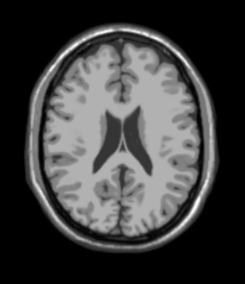
\includegraphics[width=\textwidth]{../images/screen.png}
	  \caption{Imagem Referência}
	  \label{fig:ref-image}
	\end{subfigure}
	\begin{subfigure}[t]{0.16\textwidth}
	  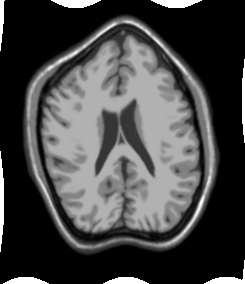
\includegraphics[width=\textwidth]{../images/movingImageSin.png}
	  \caption{Imagem Deformada Senoidal}
	  \label{fig:sin-image}
	\end{subfigure}
	\begin{subfigure}[t]{0.16\textwidth}
	  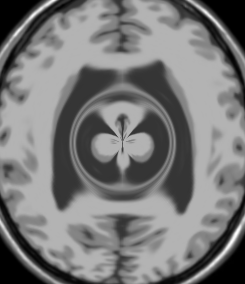
\includegraphics[width=\textwidth]{../images/movingImageDist.png}
	  \caption{Imagem Deformada pela Distância Inversa}
	  \label{fig:dist-image}
	\end{subfigure}
	\begin{subfigure}[t]{0.16\textwidth}
	  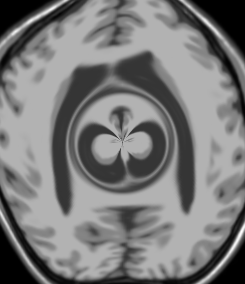
\includegraphics[width=\textwidth]{../images/movingImageSinDist.png}
	  \caption{Imagem Deformada Combinada}
	  \label{fig:sindist-image} 
	\end{subfigure} \\
	\begin{subfigure}[t]{0.16\textwidth}
	  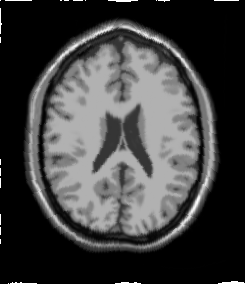
\includegraphics[width=\textwidth]{../images/resultSin.png}
	  \caption{Imagem Resultante Senoidal pelo TPS}
	  \label{fig:sin-image-tps} 
	\end{subfigure}
	\begin{subfigure}[t]{0.16\textwidth}
	  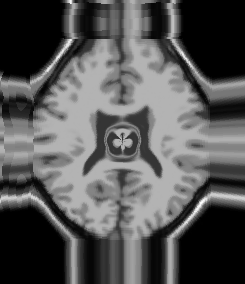
\includegraphics[width=\textwidth]{../images/resultDist.png}
	  \caption{Imagem Resultante pela Distância Inversa pelo TPS}
	  \label{fig:dist-image-tps}
	\end{subfigure}
	\begin{subfigure}[t]{0.16\textwidth}
	  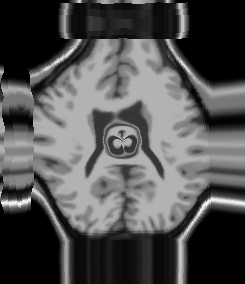
\includegraphics[width=\textwidth]{../images/resultDistSin.png}
	  \caption{Imagem Resultante pela Deformação Combinada pelo TPS}
	  \label{fig:sindist-image-tps} 
	\end{subfigure} \\
	\begin{subfigure}[t]{0.16\textwidth}
	  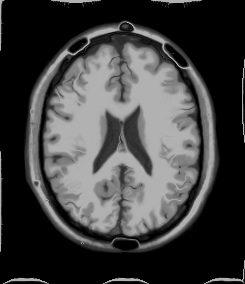
\includegraphics[width=\textwidth]{../images/resultSinDemon.png}
	  \caption{Imagem Resultante Senoidal pelo Demon}
	  \label{fig:sin-image-demon}
	\end{subfigure}
	\begin{subfigure}[t]{0.16\textwidth}
	  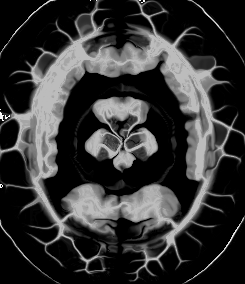
\includegraphics[width=\textwidth]{../images/resultDistDemons.png}
	  \caption{Imagem Resultante pela Distância Inversa pelo Demon}
	  \label{fig:dist-image-demon}
	\end{subfigure}
	\begin{subfigure}[t]{0.16\textwidth}
	  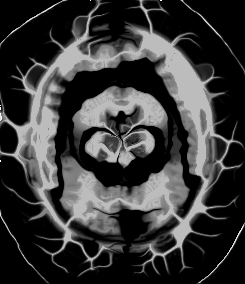
\includegraphics[width=\textwidth]{../images/resultSinDistDemon.png}
	  \caption{Imagem Resultante pela Deformação Combinada pelo Demon}
	  \label{fig:sindist-image-demon}
	\end{subfigure}
\end{figure}
	
\subsection{Resultados}
	Os resultados são bastante distintos entre os dois algoritmos, principalmente nas duas últimas deformações, que
aplicam uma deformação não uniforme nos pontos. O TPS conseguiu registrar boa parte da imagem. A deformação aplicada ao
centro foi muito intensa, logo era esperado a baixa eficácia dos algoritmos nessa região, porém o TPS se mostrou melhor
ao Demons nas regiões entorno do centro, conseguindo registrar a imagem com um certo grau de aceitação. As bordas da 
imagem ficaram com uma qualidade menor dado o método de geração das características. Quando a grade uniforme passa pela 
deformação, várias característcas ficam aglomeradas nas bordas da imagem, o que compromete o resultado nesse caso.

	Já o Demons obteve um resultado com uma qualidade inferior dado a fórmula usada para cálcular o campo vetorial.
Como vimos em (6), o Demons cálcula a direção da deformação usando o gradiente das duas imagens. Se a transformação
aplicada criar regiões com uma grande variação de gradiente o método está fadado a criar vetores que apontam para 
direções que não são ótimas, gerando os resultados acima vistos.

	A grande diferença entre o TPS e o Demons é observada no resultado com a melhor qualidade, o da deformação
senoidal. Essa deformação foi regular e as características foram geradas sem problemas, o que fez dela o caso ótimo
para os dois algoritmos. O TPS foi capaz de registrar quase que cem porcento da imagem, mesmo que acresentando um
serrilhamento resultande da interporlação. O Demons obteve um resultado um pouco pior. Os contornos da imagem foram
registrados com sucesso, contudo vários artefatos, principalmente na caixa crâniana, foram gerados, e em vários pontos
resíduos da deformação senoidal são encontrados.

\section{Conclusão}
	O TPS gerou os melhores resultados, ainda que utilizando em alguns casos um conjunto ruim de características. Dado 
o seu método que não utiliza as intensidades dos pixeis e sim marcações que indicam regiões com correspondências de 
características ele é capaz de registrar deformações que além de mover os pontos modifiquem suas intensidades. O Demons
obteve um resultado pior mas ele conta com a velocidade. Sua execução levou em torno um centésimo do levado pelo TPS. Os 
próximos passos para esse trabalho são trabalhar com a aceleração desses métodos, todos
facilmente paralelizáveis, tanto o TPS na solução do sistema linear quanto na aplicação da função de transformação, e o 
Demons com sua arquitetura altamente paralelizável, dado que os seus cálculos são totalmente locais a um pixel
\bibliography{bibliografia}   %>>>> bibliography data in report.bib
\bibliographystyle{spiebib}   %>>>> makes bibtex use spiebib.bst

\end{document} 

